% Masse kl: 4.4531 # in g (gegeben)
% Masse gr: 4.9528 # in g (gegeben)
% Durchmesser kl. Kugel: 1.5570+/-0.0010 (in cm)
% Durchmesser gr. Kugel: 1.5760+/-0.0010 (in cm)
% Volumen der kl. Kugel: 1.976+/-0.004 (in cm^3)
% Volumen der gr. Kugel: 2.050+/-0.004 (in cm^3)
% Dichte der kl. Kugel: 2.253+/-0.004 (in g/cm^3)
% Dichte der gr. Kugel: 2.416+/-0.005 (in g/cm^3)
% Gemittelte Fallzeit (hoch) kl: 12.20+/-0.13, gr: 34.75+/-0.16
% Gemittelte Fallzeit (runter) kl: 12.14+/-0.11, gr: 34.73+/-0.09
% Viskosität hoch: 1.170+/-0.013 (in mPa*s)
% Viskosität runter: 1.164+/-0.011 (in mPa*s)
% Apparaturkonstante K_gr_h: 0.02374+/-0.00030 (in mPa*cm^3/g)
% Apparaturkonstante K_gr_r: 0.02364+/-0.00025 (in mPa*cm^3/g)
% Reynoldsche Zahl Re_kl_h: 110.2+/-2.4
% Reynoldsche Zahl Re_kl_r: 111.3+/-2.0
% Reynoldsche Zahl Re_gr_h: 19.35+/-0.24
% Reynoldsche Zahl Re_gr_r: 19.46+/-0.19
%
% K_kl = 0.07640 (in m*Pa*cm^3/g) (gegeben)
% dichte_wasser = 0.998207 (in g/cm^3) (Internet)
% aus Plot:
% B = 1680+/-30
% A = 0.0038+/-0.0004
%
\section{Auswertung}
\label{sec:Auswertung}
\subsection{Viskosität von Wasser bei Raumtemperatur}
Zunächst wird die Dichte der kleinen Glaskugel $\rho_{\text{kl}}$ durch die Gleichung 
(\ref{eqn:DichtefunktionKugel}) und Gleichung (\ref{eqn:VolumenKugel}) bestimmt. 
Dafür werden die gegebene Masse $m_{\text{kl}} = 4.4531\,\unit{\gram}$ und der 
gemessenen Durchmesser $d_{\text{kl}}= \left(1.5570 \pm 0.0010\right)\,$ \unit{\centi \meter} 
verwendet.
$$\rho_{\text{kl}} = \left(2.253 \pm 0.004\right)\;\unit[per-mode=fraction]{\gram\per\cubic\centi\meter}$$ 
%
\begin{table}
  \centering
  \caption{Messdaten Kleine Kugel}
  \begin{tblr}{colspec={c c}}
      \toprule
      $t_{\text{Runter}}$ & $t_{\text{Hoch}}$ \\ 
      \midrule
      12.32 & 12.20\\
      12.18 & 12.35\\
      12.15 & 12.43\\
      12.24 & 12.23\\
      12.18 & 12.19\\
      12.18 & 12.26\\
      12.17 & 12.17\\
      11.92 & 12.10\\
      12.01 & 11.91\\
      12.07 & 12.19\\
      \bottomrule
  \end{tblr}
\end{table}
Anhand der Messdaten erhält man die folgenden Zeiten, die für die Berechnung der Viskosität benötigt werden. 
$$t_{\text{kl,r}}\left(12.14\pm0.11\right) \, \unit{\second}$$
$$t_{\text{kl,h}}\left(12.20\pm0.13\right) \, \unit{\second}$$
%
Die Viskosität von Wasser bei Raumtemperatur lässt sich mithilfe der Gleichung (\ref{eqn:EmpirischeEtaFunktion}) 
und der angegebenen Apparturkonstante der kleinen Glaskugel $K_{kl}= 0.0760 \,\unit[per-mode=fraction,inter-unit-product=\cdot]{\milli\pascal\cubic\centi\meter\per\gram}$
bestimmen.
$$\eta_{\text{Hoch}} = \left(1.170\pm0.013 \right)\, \unit[inter-unit-product=\cdot]{\milli\pascal\second}$$
$$\eta_{\text{Runter}} = \left(1.164\pm0.011 \right) \,\unit[inter-unit-product=\cdot]{\milli\pascal\second}$$
%
\subsection{Apparaturkonstante der großen Glaskugel}
Vorab wird erneut mit der Gleichung (\ref{eqn:DichtefunktionKugel}) und der Gleichung (\ref{eqn:VolumenKugel})
die Dichte der großen Glaskugel bestimmt. Hierbei beträgt die gegebene Masse $\m_{gr}=4.9528\, \unit{\gram}$ und 
der gemessene Durchmesser $d_{gr}=\left(1.5760\pm0.0010\right)\, \unit{\centi\meter}$.
$$\rho_{\text{gr}} = \left(2.416\pm0.005\right)\;\unit[per-mode=fraction]{\gram\per\cubic\centi\meter}$$ 
\begin{table}
  \centering
  \caption{Messdaten Große Kugel}
  \begin{tblr}{colspec={c c}}
      \toprule
      $t_{\text{Runter}}$ & $t_{\text{Hoch}}$ \\ 
      \midrule
      34.61 & 34.70 \\
      34.78 & 34.64 \\
      34.69 & 35.00 \\
      34.87 & 34.86 \\
      34.69 & 34.56 \\
      \bottomrule
  \end{tblr}
\end{table}
Aus den Messdaten werden folgenden Zeiten bestimmt:
$$t_{\text{gr,r}}\left( 34.73\pm0.09\right) \, \unit{\second}$$
$$t_{\text{gr,h}}\left(34.75\pm0.16 \right) \, \unit{\second}$$
Folglich wird mit der Gleichung (\ref{eqn:KFunktion}) und den zuvor berechneten Viskositäten die 
Apparaturkonstante der großen Glaskugel bestimmt.
$$K_{\text{gr,r}} = \left(0.02364\pm0.00025  \right) \, \unit[per-mode=fraction,inter-unit-product=\cdot]{\milli\pascal\cubic\centi\meter\per\gram}$$
$$K_{\text{gr,h}} = \left(0.02374\pm0.00030  \right) \, \unit[per-mode=fraction,inter-unit-product=\cdot]{\milli\pascal\cubic\centi\meter\per\gram}$$
\subsection{Bestimmung der Reynoldschen Zahl}
Durch einsetzen der Werte in die Gleichung (\label{eqn:Reynoldszahl}) ergeben sich für die 
kleine Glaskugel die folgendenen Reynoldszahlen
$$Re_{\text{kl,r}} = \left(111.3\pm2.0\right)$$
$$Re_{\text{kl,h}} = \left(110.2\pm2.4\right)$$
Analog erfogt die Berechnung der Reynoldszahlen für die große Glaskugel.
$$Re_{\text{gr,r}} = \left(19.46\pm0.19\right)$$
$$Re_{\text{gr,h}} = \left(19.35\pm0.24\right)$$
Aus den Reynoldzahlen erschließt sich, dass sowohl bei der keinen als auch bei der Glaskugeln
eine laminare Strömung entsteht.
\subsection{Temperaturabhängigkeit der Viskosität}
\begin{figure}
  \centering
  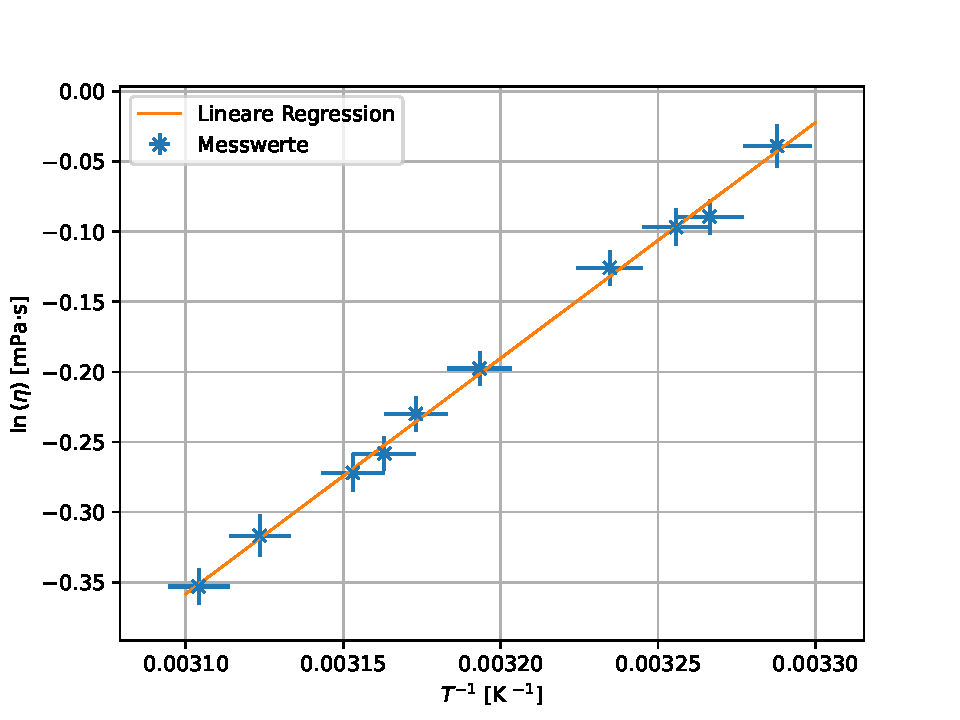
\includegraphics{plot.pdf}
  \caption{Plot.}
  \label{fig:plot}
\end{figure}

%Siehe \autoref{fig:plot}!